% This is samplepaper.tex, a sample chapter demonstrating the
% LLNCS macro package for Springer Computer Science proceedings;
% Version 2.20 of 2017/10/04
%
\documentclass[runningheads]{llncs}
%
\usepackage{float}%
\usepackage{lipsum}
\usepackage{graphicx}
\usepackage{amsmath}
\usepackage{amssymb}
\usepackage{multirow}
\usepackage{tablefootnote}
\usepackage[utf8]{inputenc} % Required for inputting international characters
\usepackage[T1]{fontenc} % Output font encoding for international characters
\usepackage[options ]{algorithm2e}
\usepackage{algorithm}% http://ctan.org/pkg/algorithm
%\usepackage{algpseudocode}% http://ctan.org/pkg/algorithmicx
\usepackage{mathpazo} % Use the Palatino font by default
\usepackage{array}% http://ctan.org/pkg/array
% Used for displaying a sample figure. If possible, figure files should
% be included in EPS format.
%
% If you use the hyperref package, please uncomment the following line
% to display URLs in blue roman font according to Springer's eBook style:
% \renewcommand\UrlFont{\color{blue}\rmfamily}

\begin{document}
%
\title{Investigation of XGBoost on Loss Functions }

%Contribution Title\thanks{Supported by organization x.}}
%
%\titlerunning{Abbreviated paper title}
% If the paper title is too long for the running head, you can set
% an abbreviated paper title here
%
\author{Rao Kotagiri\inst{1}\orcidID{a} \and
Ziren Xiao\inst{1}\orcidID{b} \and
Prafull\inst{1}\orcidID{c}}
%
% \authorrunning{F. Author et al.}
\authorrunning{Rao et al.}
% First names are abbreviated in the running head.
% If there are more than two authors, 'et al.' is used.
%
\institute{The University of Melbourne}
%
\maketitle              % typeset the header of the contribution
%
\begin{abstract}
The quantity of data we generate each day keeps on increasing. Today we are producing Exabytes of data per day, which is equal to the total data we had on earth in the year 2000. Various techniques are being used to utilize the data and gain knowledge from it. One such method is using prediction modelling in machine learning. The accuracy of these models depends on multiple factors, of which one of the critical aspects is the presence of outliers. Outliers can induce additional loss, thus reducing the accuracy of prediction, and a small variation of accuracy can sometimes lead to disastrous results. In this paper, three approaches are proposed to mitigate the effect of outliers. The first approach utilizes traditional outlier detection concepts like distance, similarity measure, cluster etc. for detecting and removing these outliers. The second approach is identifying outliers while training the model based on the error size of each trained example in the model and retraining the model. The third approach is based on the addition of user-defined loss functions, which are capable of making XGBoost model tolerable to outliers, thus lifting the requirement of removing the outliers. \\
\keywords{Outlier Detection  \and Removal \and  Loss Function \and XGBoost.}
\end{abstract}
%
%
%
\section{Introduction}

\paragraph{} In most of the prediction tasks, we analyze a tremendous amount of data. If we want to generate accurate predictions, the initial step should be mitigating the effect of outliers on the model generation. This paper proposes two different techniques for handling outliers. Approach one combines an outlier detection framework to XGBoost prediction modelling process, to discover and eliminate outliers, thus making prediction modelling more accurate for XGBoost. The method uses outlier detection techniques based on properties like distance, time-series, ensemble etc. Using this technique, we can remove erroneous data(anomalies) as well as we might be able to identify the process which leads to the outlier generation. Subsequently, the process discovery leads to the implementation of outlier detection as various services like fraud detection, malicious node identification etc. 

\paragraph{}In approach two, we replace the existing loss function for XGBoost with user-defined loss function. The new function should work in a way that it minimizes the impact of outliers on training a model, thus causing XGBoost to be more tolerant of outliers. The fundamental idea behind this approach is to design a less biased(toward outliers) loss function, compared to log loss and squared loss. XGBoost provides a few built-in loss functions like logistic regression, log squared, squared loss and hinge loss. Out of these loss functions, only Log Squared Error is sensitive to outliers, but it penalizes all data points at the same magnitude, irrespective of the size of residual. Based on these and other shortcomings, in this paper, we propose a custom loss function, which will have the advantages of Huber, Log Squared and Squared loss and will minimize their disadvantages. This methodology has a challenge that there is less prior knowledge about outliers. If required, we can overcome this problem with the use of unsupervised techniques used in approach one.

\subsection{Application}
\paragraph{Intrusion Detection System: } Information of system calls to the operating system or router is maintained in the form of logs. An anomaly in this log data can lead us to a potential attack.
\paragraph{Credit-card fraud:} There can be numerous reasons behind the loss of card credentials. If the card is used for fraud, information like purchase patterns can be used to block or detect such transactions.
\paragraph{Environmental Sensors:} Environmental data is monitored using devices; any data which deviates from the usual pattern can reveal a potential climatic threat.
\paragraph{Medical Diagnosis:} In the medical field, the data comes in many forms like images from MRI scans etc. An abnormal pattern in the image can be a disease.

\subsection{Related Work}
\paragraph{} The most common way of categorizing outliers is as local and global outliers. Global outliers are given labels 0 and 1, and local outliers have a score associated with them, the score represents the extent to which a point is an outlier. The nature of outlier detection is usually unsupervised as there is less prior knowledge about outliers.

\paragraph{} Outlier detection can also be based on the parameters of data distribution. Methods based on this, are useful for single feature datasets. Next in line are the distance-based techniques; the most popular of which is KNN. The data points are scored based on the distance similarity of a point with their neighbour. Lastly, outlier detection is also based on density-based appraoch. 


\section{Background}
\paragraph{} XGBoost is our baseline algorithm for anomaly detection and model performance improvement. As a result, the first section provides details about XGBoost and Boosting. The section also focuses on how variation in data types impacts outlier detection — followed by loss functions role in prediction modelling and outlier detection.

\subsection{XGBoost}
\paragraph{ }In 1998 a conjecture was presented by Valiant and Kearns, that raised a problem, if it was probable to combine the results from weak learners to make a strong learner. The Boosting article by Friedman and Jerome in \cite{friedman2001greedy} was the answer to this conjecture. XGBoost is an advanced and improved version of Gradient Boosting Machines \cite{chen2016xgboost}. The marked contrast between XGB and GBM is the quality of objective function, XGB objective function outperforms GBM. In the objective function of XGBoost, the regularization factor helps in handling the overfitting problem of GBM.

\paragraph{} The subsequent paragraph examines the objective function of XGBoost because the first element of the objective function(loss function), is the base of our second approach of outlier handling. The objective of XGBoost is to build regression trees in a way that it minimizes the error between the expected and true value. For this, let us consider a dataset with $n$ data points, $x$  features, target value as $y$ and predicted value as $\hat{y}_i$ for each $y$.

\begin{equation}
    \hat{y}_i = f(x_i)
\end{equation}
In the XGBoost, this function is the sum of $K$ trees on $i^{th}$ data $x_i$:
\begin{equation}
    f(x_i) = \sum^K_{k=1} f_k(x_i)
\end{equation}
where $f_k$ is calculating scores of $k^{th}$ tree using data $x_i$. An objective function can be finally represented in XGBoost as:
\begin{equation}
	Obj^*  =  -\frac{1}{2}\sum_{j=1}^T \frac{G_j^2}{H_j + \lambda} + \gamma T
\end{equation}
Where $G$ and $H$ are the gradient and hessian respectively of the loss function, $T$ is the number of leaves, and remaining symbols are regularisation constants. Our area of interest lies with the loss function mentioned above in the objective function. We are interested in designing a loss function which will make XGBoost model tolerable to outliers.

\subsection{Loss Functions}
\paragraph{} A loss function represents a cost associated with a real-time even, in terms of prediction modelling, it gives the difference between an actual value and predicted value. A single loss function can not be applied to all the problems because of the pattern of loss changes with the problem.

% \paragraph{} Least squared (LS) loss function is a popular and default loss function used in the regression. Disadvantage of using LS in the regression problems is that the LS loss function squares the error, hence in some circumstances the error largely affects the objective. For instance, since outliers typically have larger difference of predictions and observations, the errors would be magnified. As the result, a very bad score will be given to the outliers comparing with other outlier sensitive loss functions. There are many variant of the LS loss which eliminates some limitations from ordinary one. A study in have described an advanced version, Stagewise Least Square loss (SLS) function, which solves LS problem in each stage with updating a target variable, rather than using a single LS equation. It keeps the advantages from the raw function, such as simplicity and efficiency, and makes improvements like better scalability and robustness. Similarly, in, the Weight Least Square (WLS) loss function could minimise the loss function by adding a weight to each pair of the prediction and the observation.

% \paragraph{}With the aim to minimise the error from heavy tailed points, the Huber loss is an algorithm that is more sensitive to outliers. It attends to minimise the error of outliers by setting up a different function to points which are greater than a threshold and also maintains high performance for normal errors. In, it mentioned that the least square loss performs faster running speed than the Huber loss, but the variance of the least square loss is bigger in the experiment.

\subsection{Traditional Outlier Detection}


\paragraph*{Feature Selection:}  Outliers are nothing but data points based on features. The choice and quality of features help in creating an accurate model, and it also helps in identifying outliers efficiently. As a result, for identifying outliers in Link Prediction problem, we have carefully engineered features like Jaccard Coefficient, Salton Cosine etc.

\paragraph*{Proximity Based:} We can describe a data point as a proximity-based outlier if the point lies in the sparse region, i.e. it lies in a less populated area. Few simplified variations of proximity methods are a cluster, distance and density method. The outlier detection framework proposed in approach 1 utilizes 11 different detection techniques, 4 of which are based on proximity-based techniques.

\paragraph*{Outlier Ensembles for High dimensional data:} An Ensemble technique can combine multiple techniques like clustering, KNN in one design. We have used an ensemble method for high dimensional datasets where the properties of data vary with varying subspace.
\paragraph*{Outlier detection for Categorical and Timeseries data:} For Categorical Data, the similarity between values can not be identified based on the distance or separation. As a result, various domain-oriented methods exist to handle categorical data, few of which are as follows — extending the Linear model to categorical and mixed data, Proximity model for categorical data etc. In a time-series data, continuity and flow of time are robust. As the number of dimensions increases, this temporal continuity can weaken and lead to an anomaly. One of the many experiments conducted requires using time series data of energy consumption in Columbia, for forecasting energy requirements in future. Outlier detection here provides us with the insight, of power surge days in future.
%\paragraph*{Feature Selection:} The choice and quality of features help in creating an accurate model. One of the experiment is conducted on the Twitter social network dataset, implementing outlier detection on Link Prediction Problem. The engineered features Jaccard Coefficient, Salton Cosine, AA are such efficient features that individual features can help to determine node outliers.
%\paragraph*{Proximity Based:} We can describe a data point as a proximity-based outlier if the point lies in the sparse region, i.e. less populated area. Few simplified variations of proximity methods are a cluster, distance and density method. In Clustering and Density methods, the data is clustered/ grouped before outlier detection, and a new point is analysed as an outlier based on the distribution of pre-aggregated data. Whereas, in the distance-based method, the distance to the k nearest neighbour from the actual point is calculated. Proximity-based techniques are made in a way that they are capable of processing both noise and anomalies.
%\paragraph*{Outlier Ensembles for High dimensional data:} Ensembling is the method in which the output from multiple learners is combined to give the final result. An Ensemble technique can combine classification, clustering and outlier detection etc. Ensemble method is essentially useful for high dimensional datasets where the properties of data vary with varying subspace.
%\paragraph*{Outlier detection for Categorical and Timeseries data:} For Categorical Data the similarity between values can not be identified based on the distance or separation, and this creates a problem in the interpretation of such data. As a result, various domain oriented methods exist to handle categorical data, few of which are as follows. Extending the Linear model to categorical and mixed data, Proximity model for categorical data, Aggregate Statistical Similarity, The Contextual Similarity. In a time-series data, continuity and flow of time are robust. As the number of dimensions increases, this temporal continuity can weaken and lead to an anomaly.

\begin{table}[h]
\begin{center}
\begin{tabular}{|l|l|l|}
\hline
Name                       & \#sample & \#features \\ \hline
Link Prediction            &          &            \\ \hline
PJM Energy                 &          &            \\ \hline
Spatial Dataset            &          &            \\ \hline
Avocado Prices Dataset\tablefootnote{https://www.kaggle.com/neuromusic/avocado-prices}     & 14277    & 9          \\ \hline
House Sales in King County\tablefootnote{https://www.kaggle.com/harlfoxem/housesalesprediction} & 21613    & 9          \\ \hline
Medical Cost\tablefootnote{https://www.kaggle.com/mirichoi0218/insurance} & 1400    & 7         \\ \hline
Solar Radiation Prediction\tablefootnote{https://www.kaggle.com/fashionlee/using-xgboost-for-regression/data} & 36286    & 6          \\ \hline
Uniqlo Stock Price\tablefootnote{https://www.kaggle.com/daiearth22/uniqlo-fastretailing-stock-price-prediction/} & 1233    & 6          \\ \hline
\end{tabular}
\end{center}
\caption{Dataset statistics}
\end{table}

\section{Experimental Setup}
\subsection{Datasets and Source}

To evaluate the proposed approaches, we have used several datasets. Considering the limitation of space, we have provided details about seven datasets.


% \begin{enumerate}
%     \item Experiment 1 \\
%     Dataset: Link Prediction problem \\
%     Source: Kaggle/ Twitter
%     \item Experiment 2: \\
%     Dataset: PJM Energy
%     \item Experiment 4 \\
%     Dataset: Spatial Dataset \\
%     Source: UCI ML Repository
%     \item Experiment 4\\
%     House Sales in King County, USA
%     \item Experiment 5 \\
%     Medical Cost Personal \\
% \end{enumerate}



\subsection{Experiment Design}

%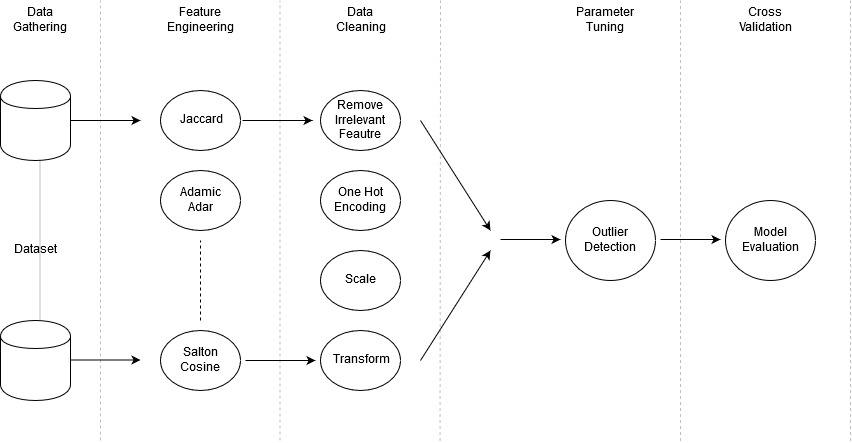
\includegraphics[scale=0.4]{hld-network.jpg} 

\paragraph{Approach 1:} In the first approach, we have integrated an outlier detection framework with XGBoost, which efficiently finds and removes outliers for various configurations. There are three different datasets used in approach one. The choice of feature influences the efficiency of an outlier detection process, we have generated quality features as and when required. Following this are the traditional machine learning steps involving removing the irrelevant features, one hot encoding where required and lastly scaling and transforming the data. Once the pre-processing of data is done, we implement the outlier detection framework, as seen in Algorithm 1 and section 4.1. The system takes input of threshold(percentage of outliers to remove) and a dictionary containing function call to all the detection techniques we want to execute and finally removes the outliers. The new dataset is then used to generate XGBoost model, which works more efficiently then the model created using the initial dataset. 

\begin{minipage}[b]{\textwidth}
    \centering
    \begin{tabular}{ccc}\hline
       
      sr	&	Category	&	Method/ Property Used \\
      \hline
    1	&	Statistical model	&	Extreme value analysis \\
    \hline
    2	&	Linear models 	&	Correlation, linear regression \\
    \hline
    3	&	Proximity based detection	&	Cluster, Distance, Density \\
    \hline
    4	&	High Dimensional detection	&	Subspace, ensemble \\
    \hline
    5	&	Outlier Ensembles	&	cluster, knn, etc. \\
    \hline
    6	&	Supervised Outlier Detection	&	Classification  \\
    \hline
    7	&	Categorical and text data	&	Extending linear, proximity model \\
    \hline
    8	&	Timeseries	&	Temporal continuity \\
    \hline
    9	&	Spatial Data	&	Behavioural and contextual attribute \\
    \hline
    10	&	Graphs and networks	&	Node and edge outlier \\
    \hline
    \end{tabular}
    \captionof{}{\\ Outlier Detection Techniques Implemented}
\end{minipage}

% evaluation methods
\paragraph{Approach 2:} In the second approach, we are using a custom loss function; the development and details of the function are present in section 4.2.  The experiment design for the approach is as follows. The propose Mixed Loss function replaces the first component(loss function) of XGBoost objective function. Experiments are conducted on different datasets, with XGBoost's inbuilt loss function and our proposed loss function. After these experiments, we aim to compare the results. To evaluate the performance of a machine learning method in a regression problem, we often use distance as the standard metric. Distance in our context means the simple error; nonetheless, this comparison of results from different datasets are difficult to compare as the results can be at different scales. Hence, we propose to use the absolute relative difference of results from our experiments. Subsequently, to compare the performance of XGBoost's default loss function and mixed loss function, we use the five-number summary, i.e. the quantile approach. Lastly, we need to aggregate the results for each dataset into one single result, and we do this by taking the mean of the top 10\% of outliers based on the error.



\section{Methodology}
\subsection{Approach 1: Proposed outlier detection framework}


\begin{algorithm}[H]
\SetAlgoLined

 \STATE $t\gets threshold\_variations$
 
 %\STATE $columns\gets [useful columns]$ 
 
 \While{$t\neq empty$}{
  \STATE $outlier\_fraction\gets t.head(1)$
  
  \STATE $classifiers\gets \{ \\
     abod: angle\_based\_outlier\_detection \\
     cblof: cluseter\_based\_outlier\_detection \\
        ... \\
  \}$
  
  %\For{$name, $object \gets 1$ to $5$}    {
  \For{$cls\_name, $cls\_object in classifiers$ $}    {
      %\State {$instance$ $\gets$ {$instances$}}
      
       %\For{$k \gets 1$ to $5$}    {
       
          %\STATE $(col_a, col_b) \gets random.sample(population=columns, k=2)$
          
          \STATE $X\_train \gets dataset$ \\
          \STATE $cls\_object.fit(X\_train)$
          
          \STATE  $scores\_pred \gets cls\_object.decision\_function(X\_train)*-1$ \\
          \STATE $y\_pred \gets cls\_object.predict(X\_train)$
          
          \STATE $outliers \gets scores\_pred.head(outlier\_fraction)$
          
          \STATE $dataset\_new \gets X\_train.drop(outliers)$
          
          \STATE $result \gets crossValidate(dataset\_new, parameters)$
          
          \STATE $y\_pred \gets xgboost.predict(dataset\_new)$
       %}
   }                
   \EndFor
 }
 \caption{Outlier Detection}
\end{algorithm}



The unique feature about the framework is that it does not require the user to run an experiment ten times in case he wants to detect outlier using ten different techniques on a single dataset. The methods start by taking in the input of the percentage of data points from the dataset, and we want to consider as outliers. The outlier fraction can be a list or a single value if it is a list the whole system iterates for all thresholds. The next step requires defining a dictionary of all the techniques we want to use on the dataset. Now, based on detection technique, the system first assigns outlier score to all data points and then based on threshold it generates labels for a point being an outlier or not.



\subsection{Approach 2: Outlier Tolerable Loss Function}

\paragraph{} XGBoost provides the flexibility of adding loss functions other than the built-in loss functions. To use a mathematical function as loss function, we need to declare a function which returns the first and second derivative of the mathematical function. The motivation behind creating the mixed loss function is, to design a function which is sensitive to small errors, but less susceptible to significant errors(outliers), we achieve this by combining squared and log square loss, which makes mixed loss tolerable to outliers.

\subsubsection{Square Loss and Log Square Loss}
Square loss squares the simple residual in prediction modelling. It is applicable on all real numbers. However, it is unstable against outliers which results into large residuals. 
\begin{align}
  f(y-\hat{y}) = (y-\hat{y})^2 \\
  f'(y - \hat{y})= -2(y-\hat{y}) \\
  f''(y - \hat{y})= 2
\end{align}
Log Square Loss is a modified version of Squared Loss. The primary purpose of this modification is stabilizing the error, and hence reducing the influence of outliers with significant errors. A drawback of the Log Squared Loss function is that the first-order differentiation is not defined when the error $y-\hat{y}$ is non-positive and the second-order derivative is not applicable at $(y-\hat{y}) = 0$. To worsen the situation if the true and predicted values are large in magnitude with large residuals, the difference of log of these values remains small. Hence, XGBoost model always counts the large value data points even with large residuals as good predictions, although they should be classified as bad predictions. Therefore, we add three features to the mixed loss function. Firstly, we use $2ln(\hat{y}-y)$ when $y-\hat{y}<0$. By calculating derivatives of this new definition and simplifying the equation, we can merge equations for $y-\hat{y} \neq 0$ into formulas below
\begin{align}
	f(y - \hat{y}) = ln((y-\hat{y})^2) = 2ln(y-\hat{y}) \\
	f'(y - \hat{y})  = -\frac{2}{y - \hat{y}} \\
	f''(y - \hat{y})  = -\frac{2}{(y - \hat{y})^2}
\end{align}
Secondly, we set derivatives to 0 if $y-\hat{y}=0$ to ensure this loss function can take all real numbers as the input. Finally, a constant coefficient $c$ is multiplied to each row of target label, if the mean value of target label is large. In this paper, $c$ is set to $\frac{mean_{target}}{10}$ if $mean_{target} > 10000$, otherwise $c=1$ which means no modification on the target label.

\subsubsection{Mixed Loss} 
Based on the shortcomings and advantages of the above loss functions, we propose a new function named as Mixed Loss. The idea behind this is that we use different loss function for a different range of residuals. If the error is less than a certain value theta, we use the square loss. Otherwise, we use the modified log squared loss function.

\begin{equation}
  f(x)=\left\{
  \begin{array}{@{}ll@{}}
    f_1(x), & x<=\theta \\
    f_2(x), & \text{otherwise}
  \end{array}\right.
\end{equation}
The threshold value $\theta$ can be determined by using smaller value of the third quartile based on the final prediction results of $f_1$ and $f_2$
\begin{equation}
    min(Q_3(f_1(y, \hat{y})), Q_3(f_2(y, \hat{y})))
\end{equation}
In this paper, we define $f_1(x)$ and $f_2(x)$ as follows
\begin{equation}
  f(x)=\left\{
  \begin{array}{@{}ll@{}}
    \text{Square Loss}, & x<=\theta \\
    \text{Log Square Loss}, & \text{otherwise}
  \end{array}\right.
\end{equation}
Because this loss function cannot be differentiated directly, we may calculate final results using the gradient and the hessian from each of the loss function separately
\begin{equation}
  f'(y - \hat{y})=\left\{
  \begin{array}{@{}ll@{}}
    -2*(y - \hat{y}), &  (y - \hat{y})<=\theta \\
    -\frac{2}{y - \hat{y}}, & \text{otherwise}
  \end{array}\right.
\end{equation}

\begin{equation}
  f''(y - \hat{y})=\left\{
  \begin{array}{@{}ll@{}}
    2, & (y - \hat{y})<=\theta \\
    \frac{2}{(y - \hat{y})^2}, & \text{otherwise}
  \end{array}\right.
\end{equation}
% The checkpoint here is that if the data is on a scale of zero to theta, then the residual will also be between zero and theta. As a result, only the Squared Error will be used. And the resultant performance of the Mixed loss will be equivalent to Squared Error. Thus the best utility of Mixed Loss is when the scale of residuals varies from $-n$ to $+n$ where $n$ is much greater than theta. 

% i don't have this case?

We expect the proposed loss function to deliver a performance between $f_1$ and $f_2$ overall. Since $f_1$ will be applied on most of the data points, the Mixed Loss will have similar performance as the $f_1$, except outliers. More importantly, the error from outliers should be lowered and smaller than $f_1$, which shows the tolerability of the new XGBoost model towards outliers. There is a scenario that Mixed Loss may not perform best: $f_1$ performs much worse than $f_2$ in most of non-outlier predictions, such as higher mean of error. In this case, Mixed Loss will still have similar result as $f_1$ but outliers are not likely to be optimised.



\section{Outcomes}
\subsection{Approach 1:}


\paragraph{} The proposed outlier detection framework integrated with XGBoost does result in improving the accuracy of prediction. The results are explained using a graph — the graphs presented below shows loss on the y-axis and outlier fraction on the x-axis. The plot shows the variation in the loss as we increase the percentage of outliers to be removed from the dataset. The experiments help us identify a trend; as we increase the outlier fraction, the trend shows that the loss first decreases and after a certain threshold, the loss again starts growing. The reduction in loss confirms our objective that XGBoost model performance improves on removing outliers using the proposed framework. After a certain point in graph loss again starts increasing, this is natural and expected, as when all the outliers have been removed, the technique starts removing useful information and hence loss increases. \\
%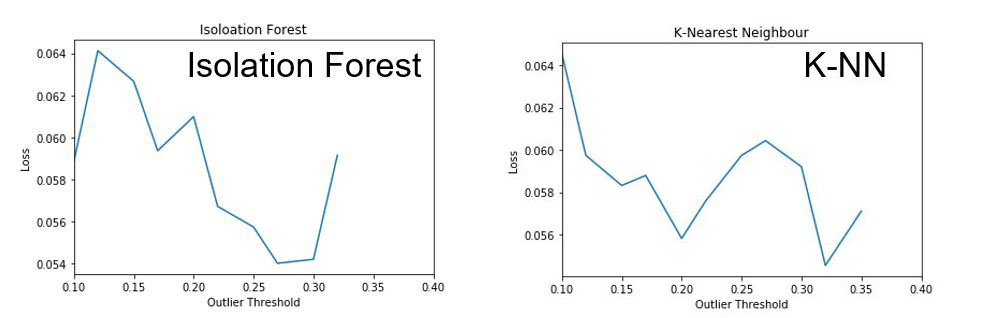
\includegraphics[scale=0.3]{tt2.jpg}

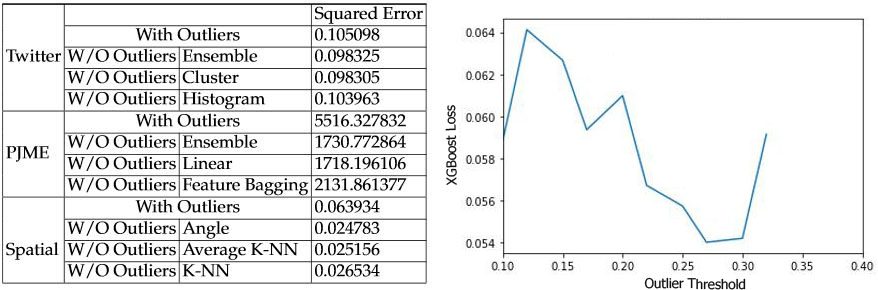
\includegraphics[scale=0.50]{result1.jpg}

\subsection{Approach 2:}
\paragraph{}

Tables \ref{5-number-summary-a2} show five-number summary statistics of 3 loss functions presented above for five datasets. Based on these summary statistics, we can see that Mixed Loss performs as we expected in the first two datasets. Specifically, (i) overall performance is between two individual loss functions (ii) maximum error is lower than Square Loss, and it is even better than the Log Square Loss in the first dataset. (iii) The mean of the top ten per cent of all errors is competitive to Squared Loss and is better than Log Squared Loss. The outcomes from (ii) and (iii) show that large errors due to outliers have been optimized. Testing on rests three datasets shows unexpected results because these are situations that $f_1$ has worse performance than $f_2$.

% \begin{table}[h]
% \begin{center}
% \begin{tabular}{|l|l|l|l|l|l|l|}
% \hline
% loss function & min & Q1 & median & Q3 & max & mean of last 10\\ \hline
% Square & 0.00004622 & 0.04750 & 0.1030 & 0.1909 & 3.607 & 0.5120\\ \hline
% Log Square & 0.00005730 & 0.1258 & 0.2494 & 0.3671 & 4.330 & 0.5677\\ \hline
% Mixed & 0.00004177 & 0.04656 & 0.1018 & 0.1871 & 2.667 & 0.4966\\ \hline
% \end{tabular}
% \end{center}
% \caption{Summary Statistics of 3 Loss Functions Based On House Sales in King County, USA Dataset}\label{summary-statistics-3-functions-k0}
% \end{table}

% \begin{table}[h]
% \begin{center}
% \begin{tabular}{|l|l|l|l|l|l|l|}
% \hline
% loss function & min & Q1 & median & Q3 & max & mean of last 10\% \\ \hline
% Square & 0.00006899 & 0.06260 & 0.1328 & 0.2303 & 0.9222 & 0.4138\\ \hline
% Log Square & 0.00007476 & 0.09142 & 0.1958 & 0.3308 & 1.074 & 0.4998\\ \hline
% Mixed & 0.00004641 & 0.06521 & 0.1367 & 0.2350 & 0.8152 & 0.4199\\ \hline
% \end{tabular}
% \end{center}
% \caption{Summary Statistics of 3 Loss Functions Based On Avocado Prices Dataset}\label{summary-statistics-3-functions-k1}
% \end{table}

\begin{table}[h]
\begin{center}
\begin{tabular}{|l|l|l|l|l|l|l|l|}
\hline
\multirow{4}{*}{Avocado}         & loss function & min        & Q1      & median & Q3     & max    & mean of last 10\% \\ \cline{2-8} 
                                 & Square        & 0.00006899 & 0.06260 & 0.1328 & 0.2303 & 0.9222 & 0.4138            \\ \cline{2-8} 
                                 & Log Square    & 0.00007476 & 0.09142 & 0.1958 & 0.3308 & 1.074  & 0.4998            \\ \cline{2-8} 
                                 & Mixed         & 0.00004641 & 0.06521 & 0.1367 & 0.2350 & 0.8152 & 0.4199            \\ \hline
\multirow{4}{*}{House Sales}     & loss function & min        & Q1      & median & Q3     & max    & mean of last 10\% \\ \cline{2-8} 
                                 & Square        & 0.00004622 & 0.04750 & 0.1030 & 0.1909 & 3.607 & 0.5120            \\ \cline{2-8} 
                                 & Log Square    & 0.00005730 & 0.1258 & 0.2494 & 0.3671 & 4.330 & 0.5677            \\ \cline{2-8} 
                                 & Mixed         & 0.00004177 & 0.04656 & 0.1018 & 0.1871 & 2.667 & 0.4966            \\ \hline
\multirow{4}{*}{Medical Cost}    & loss function & min        & Q1      & median & Q3     & max    & mean of last 10\% \\ \cline{2-8} 
                                 & Square        & 0.003483 & 0.3569 & 0.5940 & 0.9230 & 25.46        &    6.291               \\ \cline{2-8} 
                                 & Log Square    & 0.0001455 & 0.03751 & 0.08175 & 0.6444 & 0.9655  &   0.9082                \\ \cline{2-8} 
                                 & Mixed         &  0.0003314 & 0.06784 & 0.2191 & 0.7008 & 2.644        &  1.129                 \\ \hline
\multirow{4}{*}{Solar Radiation} & loss function & min        & Q1      & median & Q3     & max    & mean of last 10\% \\ \cline{2-8} 
                                 & Square        & 0.00004837 & 0.6871 & 2.647 & 13.26 & 443.4 & 106.3                  \\ \cline{2-8} 
                                 & Log Square    & 0.0001406 & 0.8509 & 0.9938 & 4.911 & 136.27 & 29.07                  \\ \cline{2-8} 
                                 & Mixed         & 0.0004841 & 0.6849 & 2.241 & 8.038 & 716.4  &  151.4                 \\ \hline
\multirow{4}{*}{Stock Price} & loss function & min        & Q1      & median & Q3     & max    & mean of last 10\% \\ \cline{2-8} 
                                 & Square        & 0.006965 & 0.2859 & 0.5966 & 0.9447 & 3.041 & 1.863                  \\ \cline{2-8} 
                                 & Log Square    & 0.0003046 & 0.1293 & 0.2494 & 0.4874 & 1.8640 &  1.036                 \\ \cline{2-8} 
                                 & Mixed         & 0.01149 & 0.3085 & 0.6205 & 0.9737 & 3.101  & 1.906                  \\ \hline
\end{tabular}
\end{center}
\caption{Results of Approach 2 On 5 Datasets}
\label{5-number-summary-a2}
\end{table}

\subsection{Comparison}
\paragraph{} In approach 1, several traditional outlier detection techniques have been used to remove outliers. With the context of the experiments conducted in this proposal, Feature bagging is highly effective in scenarios where features are numerical, and higher values can straight away identify the outliers. The Angle based technique is more suitable for large size datasets as it does not require any complicated metric; it just focuses on the variance in angles for similar points. Cluster-based methods perform exceptionally well for datasets which are clustered pattern.

\paragraph{} For the second approach, Table \ref{5-number-summary-a2} displays the results for Square, Log Square and Mixed loss. It is clear that with the change in datasets and in the worst case, Mixed loss function performs better than the default loss function of XGBoost (Square Loss) and in the majority of cases, it performs better than both the reference loss functions, as long as $f_1$ achieves our expectation.

\section{Discussion}
\subsection{Strength of proposal}
\begin{itemize}
    \item Absorbing randomness of sampling: We have validated all the models and tests using ten-fold cross-validation, it has ensured that we have used all the instances in data, both as training and test set.
    \item The Increased accuracy of prediction: Approach 1 and 2 are able to deal with variations in the dataset and make the model either tolerable to outliers or improve the accuracy of prediction.
    \item Threshold Detection: The level of anomalies, removing which influenced the accuracy of prediction in a maximum number of cases lied between 15 to 30 per cent. Also, the trend explained above, which is first lowering then increasing of loss with an increase in threshold gives us insight about the effectiveness of the technique.
    \item Overall, Mixed Loss has met our expectation. The tolerance of outliers is visible by the use of Log Square Loss to process anomalies.
\end{itemize}


\subsection{Weakness of proposal}
\begin{itemize}
    \item The time complexity of techniques goes up to the square of the number of data instances multiplied by the number of features. Especially the ensemble technique which takes in multiple techniques as input is computationally expensive.
    \item Fair Evaluation and Benchmarks: If the outlier detected was not an actual outlier, but just an error in prediction can lead us to the loss of useful information. As a result, we require a data analyst to test the outlier data instances manually. We did this work by understanding the domain of the problem and manually checked the data points.
    \item Mixed Loss function will show poor performance if the performance of $f_1$ (Square Loss) is much worse than the $f_2$ (Log Square Loss), for example, the mean of $f_1$ is much higher than in $f_2$. In this case, $f_2$ will be better almost every time and $f_1$ will be no longer necessarily needed. Thus, a replacement of $f_1$ should be considered.
\end{itemize}

\section{Conclusion}
\paragraph{} The proposal utilizes two approaches to make better predictions. The first approach aimed to use traditional outlier detection techniques for removing outliers to improve XGBoost model performance. The outcome table and graph in Section 5.1 confirms our objective by showing the improvement in the loss of XGBoost when we remove outliers using different techniques and for various threshold.


\paragraph{} Secondly, the proposal uses a user-defined mixed loss to make the model tolerant of outliers. This loss function contains two individual loss functions $f_1$ and $f_2$, which shows different sensitivity of outliers. Generally, the performance of the Mixed Loss was between $f_1$ and $f_2$. Errors of outliers are lowered because of the smaller maximum value(log). Overall, the new loss function meets our expectation by showing (i) similar performance as $f_1$ (ii) and tolerance to outliers.

\paragraph{} Both techniques are efficient when it comes to detecting and removing outliers. As a result, the proposal is able to improve the accuracy of prediction for XGBoost. Lastly, there needs to be a comparison made between approach one and two. There is a risk associated with Approach 1 when we remove the outlier points, upward spikes are observed in graph of section 5.1, which is an increase in loss, and it shows that along with outliers useful information is also being removed. Whereas Approach 2 lifts the requirement of removing outlier, it works by penalizing the outlier and hence making it a more efficient technique.

% Prafull's future work


% Ziren's future work
\section{Future Work} For future directions and further improvements, we propose three key points. The first direction we aim is to replace the Squared Loss in Mixed Loss because Square Loss performed worse than the Log Square Loss for most of the data. The replacement function should satisfy the following conditions. First, it should be less sensitive to outliers; second, it should accept all real numbers as the input. Third it should be suitable for regression problems, instead of focusing on classifications and lastly, the performance should be better than the Log Square Loss in predicting non-outliers.


%
% the environments 'definition', 'lemma', 'proposition', 'corollary',
% 'remark', and 'example' are defined in the LLNCS documentclass as well.
%

%
% ---- Bibliography ----
%
% BibTeX users should specify bibliography style 'splncs04'.
% References will then be sorted and formatted in the correct style.
%
\bibliographystyle{splncs04}
\bibliography{bib}
%

\end{document}
